\section{Einleitung}
Wenn Kräfte $F_{\symup{i}}$ auf einen Körper wirken, kann es bei hinreichender Kraft zu einer Deformierung des Körpers kommen. Das Elastizitätsmodul $E$ ist eine Kenngröße dieser Deformation und wird in diesem Versuch für zwei Aluminiumkörper bestimmt.

\section{Theorie}
\label{sec:Theorie}

\subsection{Das Hooksche Gesetz}
\label{sec:hook}
In dem Fall, dass eine auf einen Körper wirkende Spannung eine hinreichend kleine Änderung einer Körperdimension 
$\frac{\Delta L}{L}$ bewirkt, besteht ein linearer Zusammenhang zwischen der Spannung, der durch das 
\textit{Hooksche Gesetz}(\autoref{eq:hook}) beschrieben wird. Der Proportionalitätsfaktor $E$ wird als Elastizitätsmodul 
definiert und ist eine material- und formabhängige Konstante.
\begin{equation}
    \sigma = E \cdot \frac{\Delta L} {L}
    \label{eq:hook}
\end{equation}

\subsection{Durchbiegung eines Stabes bei einseitiger Einspannung}
Wird ein Stab, wie in \autoref{fig:stab einseitig eingespannt} zu sehen, einseitig eingespannt, verbiegt es sich bereits 
unter seinem Eigengewicht. An jeder Stelle $x$ des Stabes kann eine Durchbiegung $D(x)$ festgestellt werden.
Wird weiteres Gewicht an ein Stabende angehängt, wirkt eine größere Gewichtskraft $F_{\symup{G}}$ und der Stab 
verbiegt sich nochmals mehr und die Durchbiegung $D(x)$ wird an jeder Stelle $x$ größer.
\begin{figure}
    \centering
    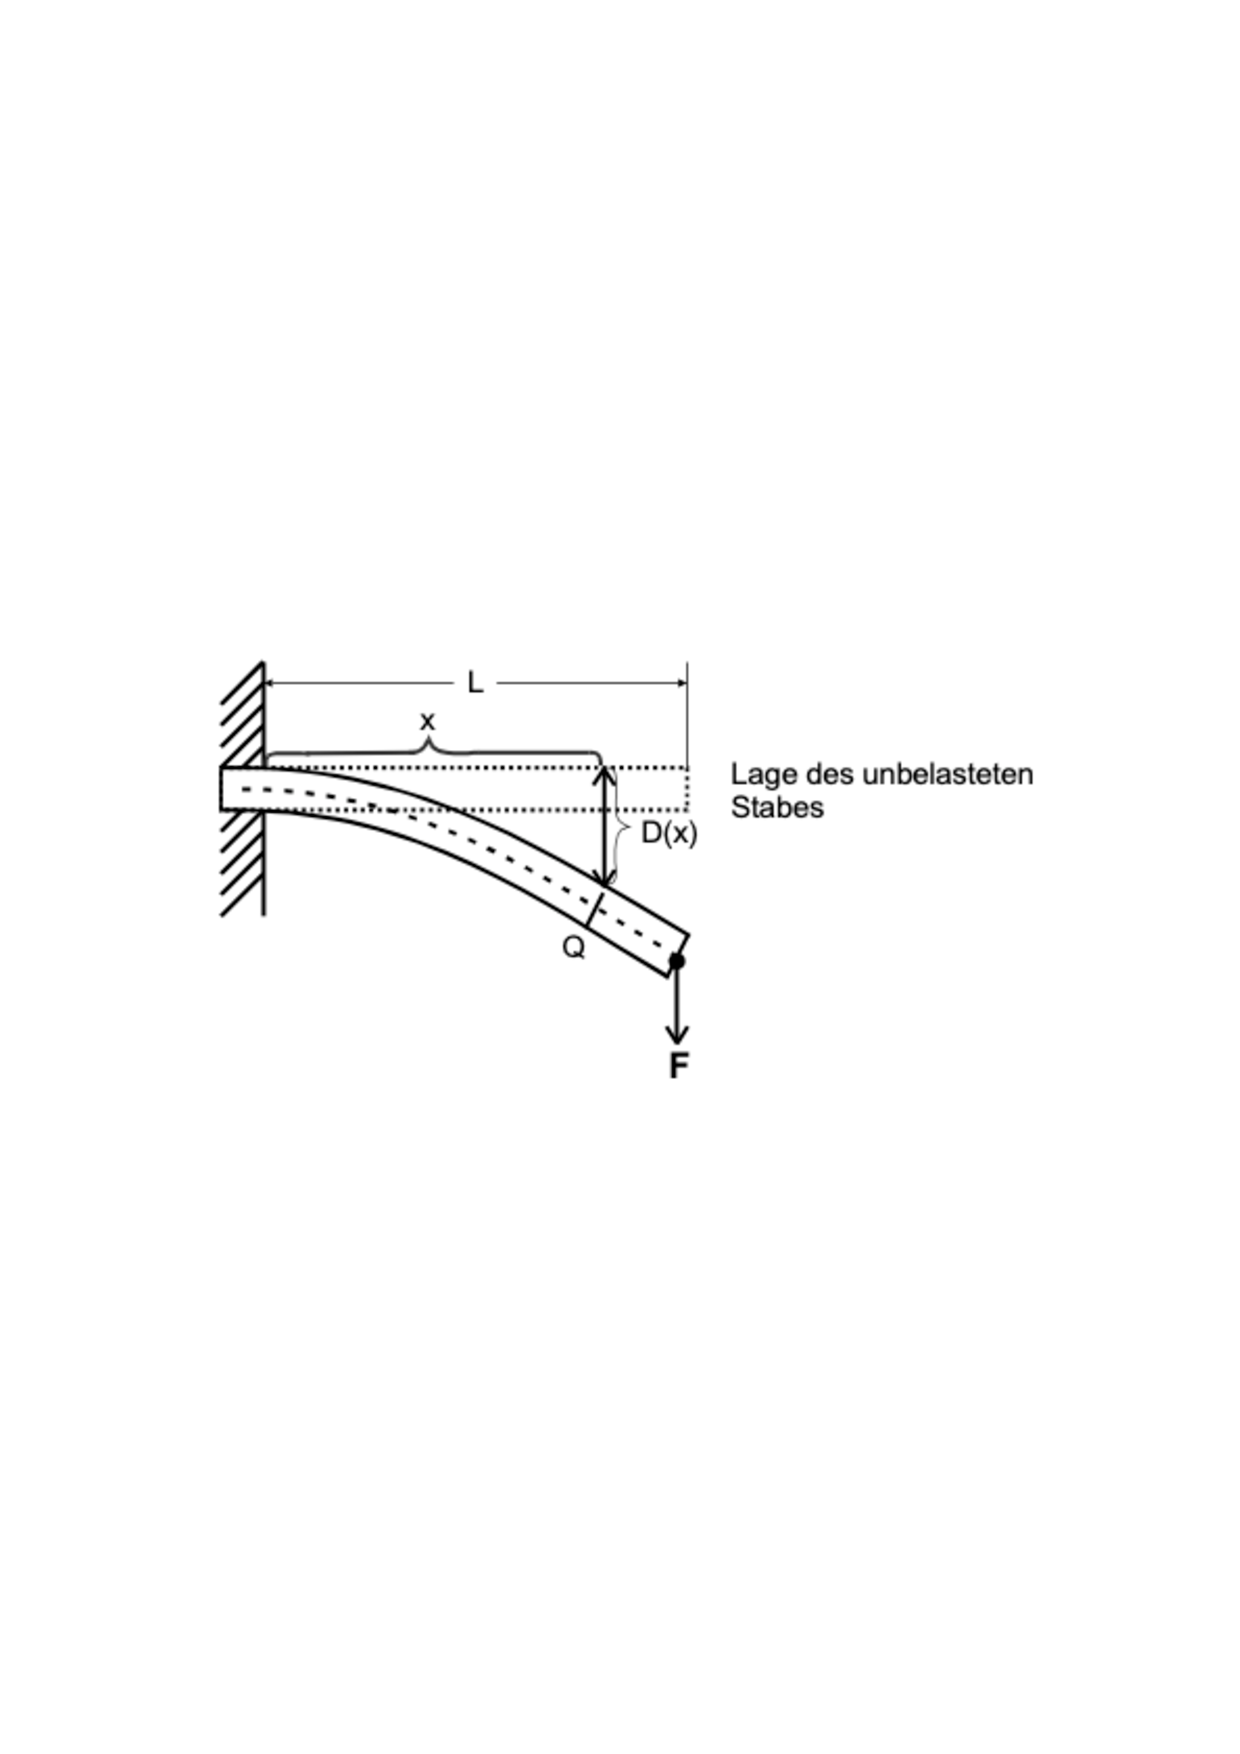
\includegraphics[height=6cm]{content/Abbildungen/stab_einseitig_eingespannt.pdf}
    \caption{Einseitig eingespannter Stab. \cite{v103}}
    \label{fig:stab einseitig eingespannt}
\end{figure}

Die wirkende Gewichtskraft $F_{\symup{G}}$ hat zur Folge, dass in dem Stab Drehmomente $M$ wirken, die den Stab aus seiner 
Ruhelage verdrehen. Diesen Drehmomente $M$ gegenüber treten Normalenspannungen auf und es stellt sich ein 
Gleichgewichtszustand mit endgültiger Durchbiegung $D(x)$ ein. Der obere Teil wird durch vorhandene Zugspannungen 
gestreckt während der untere Teil durch Druckspannungen gestaucht wird. Zwischen diesen Teilen liegt eine Fläche, die 
ihre ursprüngliche Länge beibehält und als \textit{neutrale Phase} bezeichnet wird. Die Zug- und Druckspannungen $\sigma$, 
welche an der neutralen Phase angereifen, sind genau entgegengesetzt und heben sich daher auf. 
Die \autoref{fig:neutrale phase} verdeutlicht dies.

\begin{figure}
    \centering
    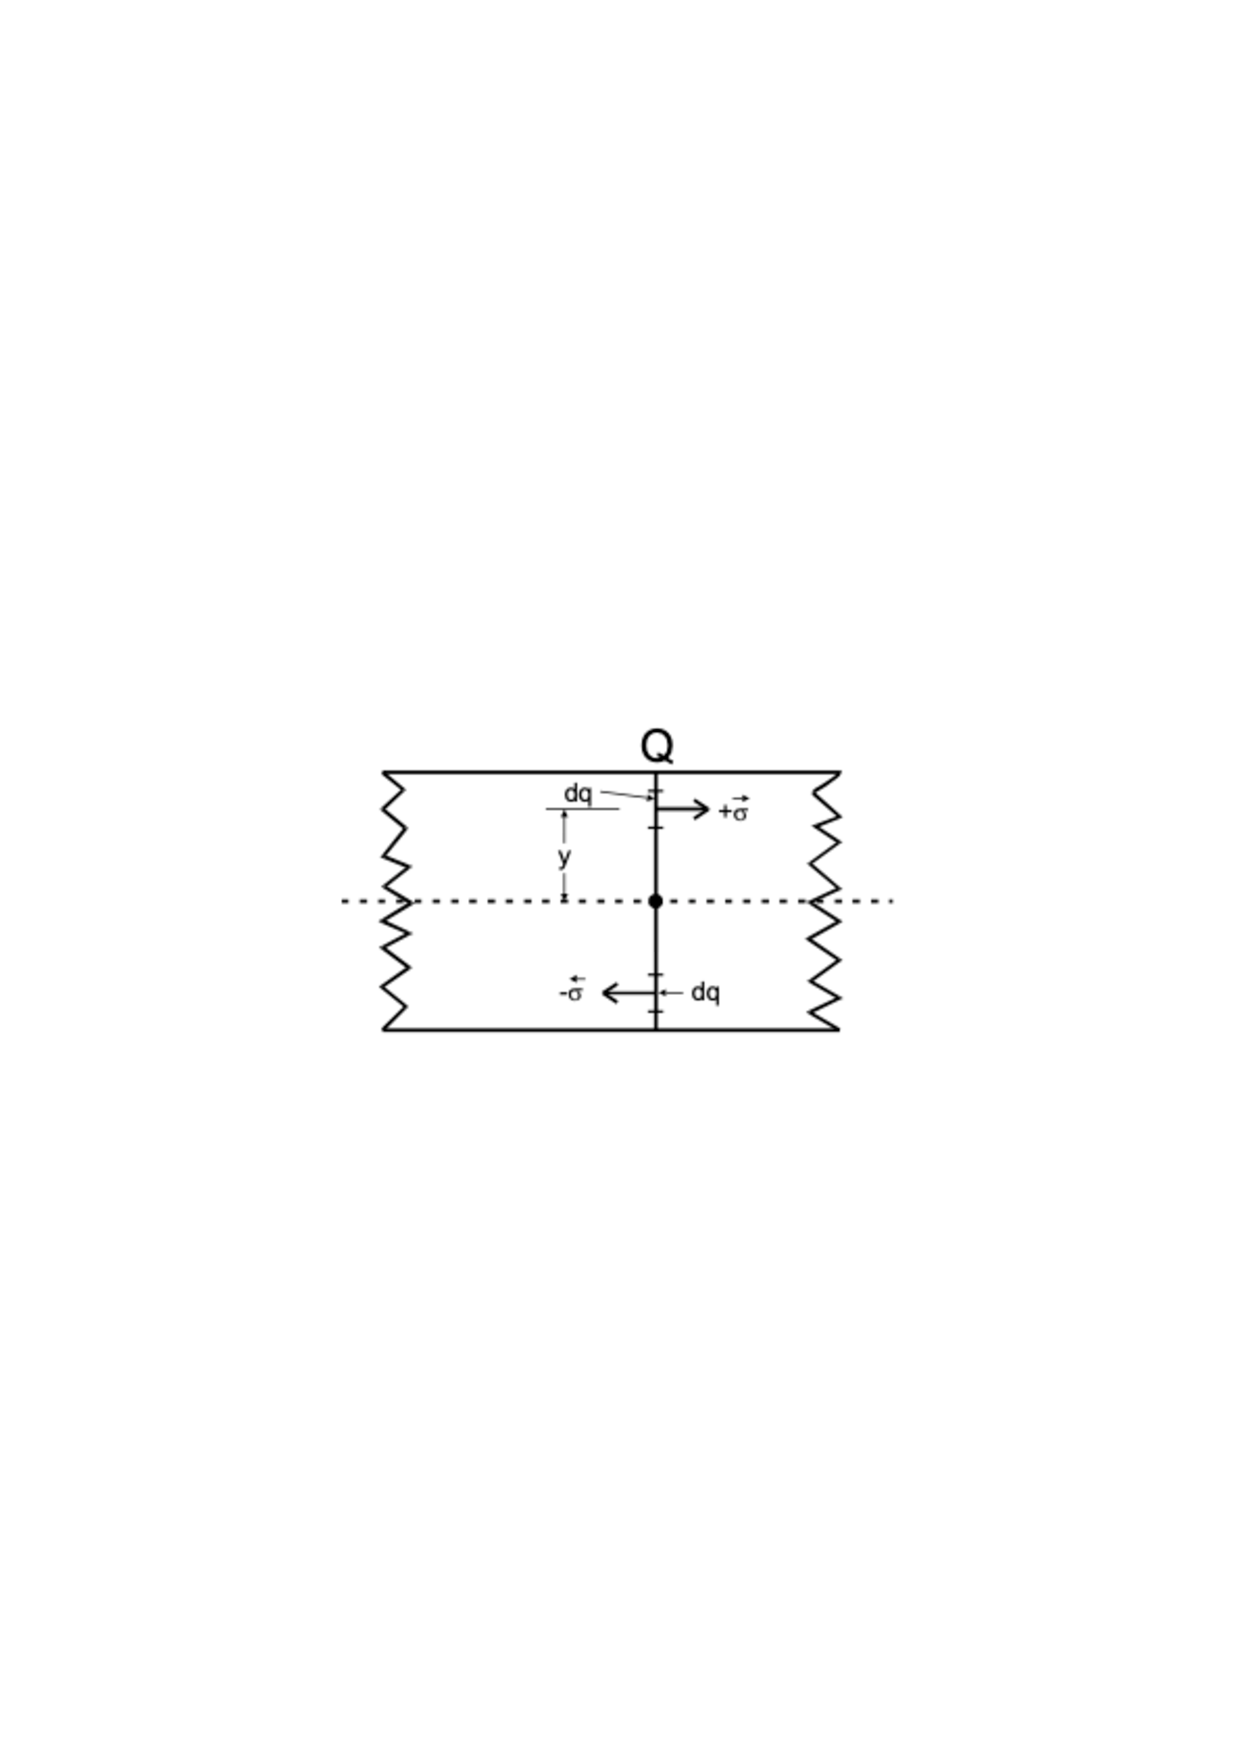
\includegraphics[height=6cm]{content/Abbildungen/neutrale_phase.pdf}
    \caption{Neutrale Phase Q mit wirkenden Zug- und Druckspannungen $\sigma$. \cite{v103}}
    \label{fig:neutrale phase}
\end{figure}

Das an der neutralen Phase $Q$ wirkende Drehmoment lässt sich also schreiben als:
\begin{equation}
    M_{\symup{\sigma}}=\int_{Q}y\sigma(y)\symup{d}q
    \label{eq:drehmoment neutrale phase}
\end{equation}
Hierbei bezeichnet $y$ den Abstand des Flächenelements d$q$ von der neutralen Phase $x$ und $Q$ einen Querschnitt des Körpers.


